\documentclass[11pt]{article}

\usepackage[margin=1in]{geometry}
\usepackage{booktabs}
\usepackage{amsmath,amssymb}
\usepackage{microtype}
\usepackage{natbib}
\usepackage{graphicx}
\usepackage{xcolor}
\usepackage{pgfplots}
\pgfplotsset{compat=1.18}
\usepackage{float}
\usepackage{listings}
\usepackage[colorlinks=true,linkcolor=black,citecolor=black,urlcolor=blue]{hyperref}

\newcommand{\stddeck}{\textsc{Standard}}
\newcommand{\intdeck}{\textsc{Interactive}}
\newcommand{\searchn}[1]{\textsc{search}-#1}
\newcommand{\ci}[2]{\,[#1,\,#2]}
% Challenges carry their own counter so \ref yields "Challenge 3", not "Challenge 6.3".
\newcounter{challenge}
\renewcommand{\thechallenge}{\arabic{challenge}}
\newcommand{\challenge}[2]{%
  \refstepcounter{challenge}%
  \subsection*{Challenge \thechallenge: #1}\label{#2}}

% Long unbreakable \texttt{} identifiers (Ability::Triggered, OnNthResolutionThisTurn)
% cannot be hyphenated; let TeX stretch interword space rather than overrun the margin.
\setlength{\emergencystretch}{3em}

\lstset{
  basicstyle=\ttfamily\footnotesize,
  keywordstyle=\color{blue!55!black},
  commentstyle=\color{gray},
  stringstyle=\color{green!40!black},
  showstringspaces=false,
  language=Python,
  frame=single, framesep=5pt, rulecolor=\color{gray!45},
  breaklines=true,
}

\title{\textbf{manabot}: A Research Platform and Open Challenge Set\\ for \textit{Magic: The Gathering}}

\author{Jack Heart\\ \small Loopflow Studio}

\date{\today\\[0.5em]\small\textit{Working draft --- a standing snapshot of the platform and the open frontier.}}

\begin{document}
\maketitle

\begin{abstract}
\textit{Magic: The Gathering} has an open, unbounded card pool, hidden information with a \emph{structured and enumerable} belief space, action sets whose size and meaning change at every decision, and Turing-complete rules. It is among the most difficult games that remains genuinely unsolved, and it has lacked the thing that made Go, poker, and \textit{StarCraft} tractable as research programs: a fast, honest, instrumented environment with calibrated baselines.

This paper presents \textbf{manabot}, that environment. We contribute (i) \textbf{managym}, a deterministic, seedable, forkable Rust engine ($\approx$10.7k lines, 106 rules-cited tests) that runs $1.8\times10^{5}$ steps/second and exposes belief-state determinization as a native primitive, making imperfect-information search a one-line call; (ii) a \textbf{calibrated measurement protocol} --- seat-balanced evaluation, Wilson intervals, pre-registered predictions, and a cost axis in dollars --- without which, we show, win rates in this domain measure seating rather than skill; (iii) a \textbf{reference baseline suite} spanning a \$0 flat determinized search, PPO under three reward regimes, and a distilled search policy, each with its strength located on a common ladder; and (iv) a statement of \textbf{five open challenge areas}, each with a current best number, an entry criterion, and the specific reason we believe it is now approachable.

The headline for a prospective entrant is uncomfortable and clarifying: at present, \emph{a search that costs nothing to train and seven milliseconds to run defeats every policy we have trained}, and behavior cloning from that search is roughly six times more cost-effective than reinforcement learning from scratch. The learning half of this problem is wide open. We have built the instrument; the science has not been done.
\end{abstract}

\section{Introduction}

Every domain that became a productive arena for sequential decision-making research got there the same way: someone built a fast simulator, someone else established that a given number meant something, and only then did algorithms accumulate. ALE, the Gym suite, OpenSpiel, and the poker benchmarks all follow this shape. The environment is not scaffolding around the science; for a period, it \emph{is} the science.

\textit{Magic: The Gathering} has not had this. It is a natural target --- it is imperfect-information, it is long-horizon, its rules are Turing complete \citep{churchill2019turing}, and, uniquely among the hard card games, \emph{its hidden state is exactly enumerable}, because in constructed play both decklists are public knowledge. The belief space is a distribution over multisets drawn from a known pool. That is a far friendlier object than the abstraction-and-blueprint machinery poker required, and it means the imperfect-information content of \textit{Magic} is directly attackable with modern methods. Yet published work on \textit{Magic} is thin, and the most relevant search result is over a decade old \citep{cowling2012magic}.

We believe the reason is that the entry cost is brutal. A researcher who wants to study belief modeling in \textit{Magic} must first write a rules engine, which is a multi-year project with no publications in it; must then discover, painfully, that the obvious way to evaluate an agent in this game is contaminated; and must then find that their learned policy is worse than a trivial search they could have written in an afternoon. We know this because we did all three, in that order.

This paper is an attempt to pay that cost once, publicly, so that the next person does not have to. Sections \ref{sec:platform}--\ref{sec:protocol} describe the platform and the measurement protocol. Section \ref{sec:baselines} gives the reference baselines --- what currently works, what it costs, and where each agent sits on a common strength ladder. Section \ref{sec:challenges}, the core of the paper, states the five challenge areas we believe define the frontier, each with an entry criterion an incoming researcher can aim at. Section \ref{sec:pitfalls} records the calibration findings that will otherwise cost every entrant the same months they cost us.

\paragraph{What we are claiming.} That the environment is fast, correct within a stated subset, and instrumented; that the protocol is sound; that the baselines are honestly measured; and that the five challenges are the right ones. We are explicitly \emph{not} claiming to have trained a strong agent. We have not. That is the invitation.

\section{Why \textit{Magic} Is Hard, Precisely}
\label{sec:why}

Difficulty claims about games are cheap. Here is what is actually load-bearing about this one, in the form of the constraints each property places on a solution.

\paragraph{The action set is variable, state-dependent, and object-referential.} At each decision the legal set is a list --- cast this, block that with this, target the other --- of size $1$ to $20$ in our subset, and index $i$ carries no meaning across states. A policy cannot have an output head per action. It must score actions by \emph{what they do to which objects}, which forces object-centric architectures and rules out most of the standard toolbox. The mean is $3.08$ valid actions per decision, but the tail is what matters.

\paragraph{The hidden state is enumerable, and nobody has exploited that.} Both decklists are public. The unknown is precisely the opponent's hand plus both library orderings. A uniform draw from the opponent's unseen pool is therefore an \emph{exactly correct} posterior at turn one --- and increasingly wrong thereafter, because a player who has not cast \textit{Counterspell} in four turns is more likely to be holding one. This is a clean, well-posed belief-modeling problem with a tractable prior and an obvious source of learning signal. It is Challenge \ref{ch:belief}, and we consider it the single most interesting thing about the domain.

\paragraph{The horizon is six times the credit window.} Games run 33--41 turns and surface $117$--$194$ decisions. A PPO learner with $\gamma=0.99$, $\lambda=0.95$ has an effective GAE horizon of $1/(1-\gamma\lambda)\approx16.8$ steps. Credit for winning must therefore travel roughly six horizons. The obvious fix --- dense reward shaping --- is, we show in \S\ref{sec:pitfalls}, actively harmful. So the horizon problem must be solved architecturally, and it is unsolved.

\paragraph{The card pool is open and semantic.} We implement 35 cards. \textit{Magic} has tens of thousands, and new ones ship quarterly with mechanics that did not previously exist. A tabular or index-based policy is definitionally a dead end. Whatever wins here must read a card and know what it does --- which, in 2026, is a suggestive statement. This is Challenge \ref{ch:pool}.

\paragraph{The variance is enormous and the confounds are worse.} Between two \emph{uniformly random} players on a creature deck, going first wins $94.1\%\ci{92.5\%}{95.4\%}$ of games. Any evaluation that does not balance seats is measuring the seat. We discovered this after it had invalidated our own founding result (\S\ref{sec:pitfalls}).

\section{The Platform}
\label{sec:platform}

\subsection{managym: the engine}

A two-player subset of the \textit{Comprehensive Rules} in Rust ($\approx$10{,}738 lines), with PyO3 bindings. Table~\ref{tab:rules} states coverage exactly, because a benchmark whose scope is vague is not a benchmark. The subset is closed: everything in it is tested, and no card in the pool depends on anything outside it.

\begin{table}[H]
\centering\small
\begin{tabular}{llp{6.4cm}}
\toprule
\textbf{CR section} & \textbf{Status} & \textbf{Notes / known gap} \\
\midrule
103 Game start & tested & Opening hand of seven; \textbf{no mulligans} \\
106 Mana & tested & Deterministic auto-tap; no floating-mana choice \\
117 Priority & tested & APNAP pass loop \\
305 Lands & tested & One per turn; no additional-land effects \\
601 Casting (subset) & tested & Timing/cost legality for the current pool \\
508/509 Attack, block & tested & Per-creature declaration; \textbf{single-block only} \\
510 Combat damage & tested & First/double strike, trample, deathtouch, menace \\
514, 704.5 Cleanup, SBAs & tested & Life, empty draw, lethal damage, token cleanup \\
603 Triggers & tested & Data-driven substrate; \S\ref{sec:triggers} \\
\midrule
Layers, replacement/prevention & \textbf{absent} & Designed, unimplemented. Challenge \ref{ch:rules} \\
Multiplayer, planeswalkers, battles & \textbf{absent} & \texttt{Game::new} asserts two players \\
\bottomrule
\end{tabular}
\caption{Rules coverage. ``Tested'' means a CR-cited integration test exists under \texttt{managym/tests/rules/}; there are 106 of them. The absences bound every claim in this paper and constitute part of the open work.}
\label{tab:rules}
\end{table}

The pool is 35 cards: five basic lands, 18 from Alpha (\textit{Lightning Bolt}, \textit{Counterspell}, \textit{Ancestral Recall}, \textit{Shivan Dragon}, \ldots), \textit{Pyroclasm}, \textit{Man-o'-War}, and a ten-card modern slice exercising tokens, $+1/+1$ counters, flash, and ETB triggers with subject predicates. Two decklists are standard:

\begin{itemize}\itemsep1pt
\item \stddeck{} --- 12 Mountain, 12 Forest, 18 Llanowar Elves, 18 Grey Ogre. Zero interaction: a pure race.
\item \intdeck{} --- 12 Island, 12 Mountain, 20 creatures, 16 interaction spells (6 \textit{Lightning Bolt}, 4 \textit{Counterspell}, 3 \textit{Ancestral Recall}, 3 \textit{Pyroclasm}). Instants make timing matter.
\end{itemize}

Having two decks with opposite strategic character is not decoration. We show in \S\ref{sec:pitfalls} that an agent trained with terminal reward alone plays them differently --- casting nearly always on one, holding nearly always on the other --- and that this is the sharpest available test of whether a learner has learned the game or memorized a habit.

\subsection{Determinization as a primitive}
\label{sec:determinize}

This is the design decision that makes the platform useful for imperfect-information research. All randomness flows through one \texttt{ChaCha8Rng}, so \texttt{(decklists, seed)} determines a game exactly. \texttt{Env::fork()} deep-clones an independent game. And \texttt{determinize(seed, perspective)} samples from the belief state directly: it pools the opponent's hand with their library, shuffles, re-deals to preserve the observed hand size, reshuffles the perspective player's library, and preserves every public zone and the current action space.

On top of this the engine ships \texttt{flat\_mc\_scores}, which for each legal action samples $W$ determinized worlds, applies the action to a clone, and scores by $R$ uniform playouts to a true terminal, sharing worlds across actions as common random numbers. \textbf{Search is an engine primitive, not a Python loop.} This is why the search experiments in \S\ref{sec:baselines} cost 4.5 CPU-core-hours rather than a week, and it is the hook on which we expect Challenge \ref{ch:belief} to hang: replacing the uniform resample inside \texttt{determinize} with a learned posterior is a local change to one function.

\begin{lstlisting}[caption={The whole imperfect-information API. Signatures are current as of this draft.}]
import managym

hero    = managym.PlayerConfig("hero",    {"Mountain": 12, "Grey Ogre": 18, ...})
villain = managym.PlayerConfig("villain", {"Island": 12, "Counterspell": 4, ...})

env = managym.Env(seed=0, skip_trivial=True)
obs, info = env.reset([hero, villain])

while not obs.game_over:
    # One line of imperfect-information search: 16 worlds x 4 rollouts per
    # legal action, scored by uniform playouts to a true terminal.
    scores = env.flat_mc_scores(worlds=16, rollouts=4, seed=1, max_steps=2000)
    obs, reward, terminated, truncated, info = env.step(argmax(scores))

# Or drive the belief state yourself:
scratch = env.fork()               # independent deep clone
scratch.determinize(seed=7)        # resample opponent hand + library orders
scratch.random_playout(seed=7)     # uniform rollout to terminal
\end{lstlisting}

\subsection{Throughput, and where the time actually goes}

Measured on an Apple M4 Max. Environment stepping alone: $90{,}898$ steps/s at one environment, $183{,}350\pm660$ at sixteen, saturating near $1.9\times10^{5}$. Add policy inference and this collapses to $2{,}035$ steps/s; add the full PPO update and it is $2{,}472$--$2{,}856$.

\textbf{The environment is not the bottleneck, and has not been since early 2026.} Inference costs roughly $72\times$ the environment step. We flag this because it inverts the assumption most board-game RL tooling is built on, and because it means an entrant's compute budget is spent almost entirely on their own network. The engine will not be what limits you.

\subsection{The trigger substrate}
\label{sec:triggers}

Triggered abilities are data, not code: \texttt{Ability::Triggered\{condition, effects\}}, where \texttt{TriggerCondition} ranges over ETB / dies / attacks / becomes-tapped / tapped-for-mana / upkeep / ``you draw your $n$th card this turn'', each parameterized by a \texttt{TriggerSubject} (\texttt{This}, \texttt{AnotherYouControl(pred)}, \texttt{AnyYouControl(pred)}) over a structural \texttt{CardPredicate}. Effects compose, including a recursive \texttt{OnNthResolutionThisTurn} gate. Triggers are collected from game events, ordered APNAP, dropped when no legal target exists (CR 603.3d), and placed on the stack.

This substrate is the bet on which card-pool growth rests. Whether it generalizes past 35 cards is untested, and is Challenge \ref{ch:rules}.

\subsection{manabot: the learning side}

A Gymnasium-compatible vectorized wrapper \citep{towers2024gymnasium}, one shared observation encoder, and three consumers of it: a PPO learner, a flat-MC search player, and a distillation harness.

\paragraph{Observations} are hidden-information correct --- the opponent's hand and both libraries are never encoded --- and object-centric: per-player $[27]$, per-card $[60\times33]$, per-permanent $[30\times7]$, actions $[20\times8]$, events $[32\times7]$, plus \texttt{action\_focus} $[20\times2]$, which maps each action to the (up to two) objects it refers to. Validity masks accompany every padded tensor.

\paragraph{The policy} embeds each object class into $d=64$, optionally mixes them with one transformer block \citep{vaswani2017attention} carrying a learned \emph{perspective} vector whose sign flips by ownership, then scores each action by concatenating its embedding with those of its focus objects and passing the result through a shared head. One logit per action slot; invalid slots masked to $-10^8$. It is deliberately \emph{not} a pointer network \citep{vinyals2015pointer}. 100{,}354 parameters (50{,}306 without attention). We regard this architecture as a placeholder, not a contribution.

\paragraph{PPO} is CleanRL-style \citep{huang2022cleanrl,schulman2017ppo} with GAE \citep{schulman2015gae}: $\gamma=0.99$, $\lambda=0.95$, lr $2.5\times10^{-4}$ annealed, 16 envs $\times$ 128 steps, 4 minibatches, 4 epochs, clip $0.1$. Three reward regimes are selectable: terminal-only; per-event (``pay-per-event'': $+0.03$ land, $+0.06$ creature, $+0.01$ per point of opponent life); and potential-based \citep{ng1999shaping}, $\gamma\Phi(s')-\Phi(s)$ with matched weights. \S\ref{sec:pitfalls} reports which of these you should use, and the answer is not the one we shipped first.

\paragraph{Search and distillation.} \texttt{FlatMCPlayer} exposes a single strength dial $N$ = simulations per legal action. Distillation is pure behavior cloning from \searchn{64} self-play: record every decision as (observation, teacher's $\arg\max$), minimize cross-entropy through the student's masked logits, split train/validation \emph{by game}. No DAgger \citep{ross2011dagger}, no soft targets, no value head --- all three are open.

\section{The Measurement Protocol}
\label{sec:protocol}

We state this before the results because in this domain it \emph{is} a result, and because an entrant who ignores it will produce numbers that do not mean anything. We know, because we did.

\paragraph{Seat balancing is mandatory.} The engine gives \texttt{PlayerId(0)} the first turn. Between two uniformly random players:

\begin{center}\small
\begin{tabular}{lccc}
\toprule
Deck & On the play & On the draw & Overall (balanced) \\
\midrule
\stddeck  & $94.1\%\ci{92.5}{95.4}$ & $5.9\%$ & $50.3\%\ci{47.2}{53.4}$ \\
\intdeck  & $23.1\%\ci{20.6}{25.8}$ & $76.9\%$ & $48.9\%\ci{45.8}{52.0}$ \\
\bottomrule
\end{tabular}
\end{center}

On the creature deck, moving first wins $94\%$ of games between two agents with no policy at all. On the interactive deck the advantage \emph{inverts} --- a random agent on the play walks its creatures into an untapped opponent. Either way, an unbalanced win rate is a reading of the seat. All numbers in this paper alternate the hero between seats and report overall and per-seat rates with Wilson intervals \citep{wilson1927}.

\paragraph{The gate.} A policy \emph{passes} if, over $\ge400$ seat-balanced games against a uniform random opponent on \intdeck, its Wilson $95\%$ lower bound exceeds $55\%$ overall \emph{and} its win rate exceeds $50\%$ in each seat separately. The second clause exists to reject seat-parasitic policies, which we produced immediately upon looking for them.

\paragraph{Ladder strength.} Win rate against random saturates and cannot rank strong agents. We therefore index strength by \textbf{ladder strength}: the largest $N$ such that a policy, alone and without search at inference time, beats \searchn{N} head-to-head. The ladder is training-free, reproducible, and monotone --- we verify that \searchn{256} beats \searchn{16} $76.7\%\ci{71.6}{81.1}$ --- and $N$ is directly interpretable as \emph{how much thinking this policy is worth}. It is the primary metric of this benchmark.

\paragraph{The cost axis.} Strength is meaningless unbudgeted. We book compute at the AWS \texttt{g5.xlarge} on-demand rate (\$1.006/hr); at the measured throughput of the era, $10^{6}$ training steps $=$ \$0.44. This is a portable fiction: everything actually ran on one laptop, and the true marginal cost of the entire program was a few dollars of electricity. We keep the fiction because strength-per-dollar comparisons need a common denominator, and we label it a fiction rather than launder it.

\paragraph{Pre-registration.} Each experimental cycle opens with a written question, a prediction, and a cost cap, and closes with a report in \texttt{reports/} recording whether the prediction held. Of seven predictions registered so far, three were refuted outright. We publish all of them.

\section{Reference Baselines}
\label{sec:baselines}

\begin{figure}[t]
\centering
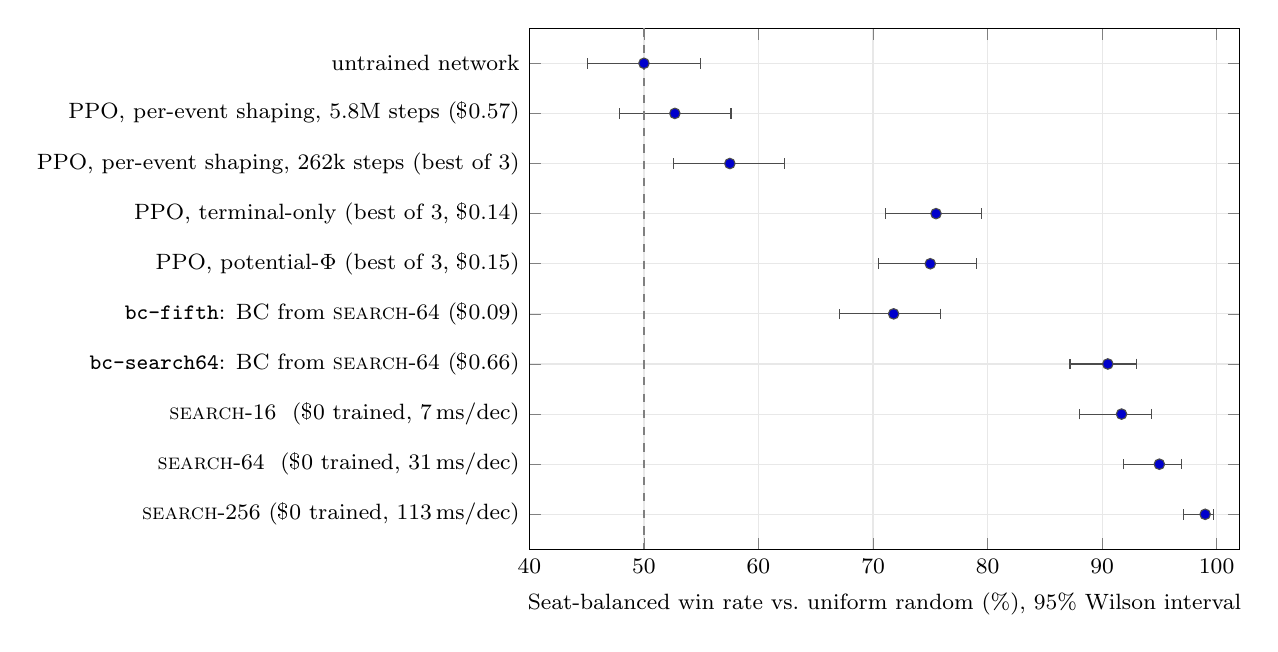
\begin{tikzpicture}
\begin{axis}[
  width=10.6cm, height=8.2cm,
  xlabel={Seat-balanced win rate vs.\ uniform random (\%), 95\% Wilson interval},
  xmin=40, xmax=102,
  ytick={0,...,9},
  yticklabels={
    {untrained network},
    {PPO, per-event shaping, 5.8M steps (\$0.57)},
    {PPO, per-event shaping, 262k steps (best of 3)},
    {PPO, terminal-only (best of 3, \$0.14)},
    {PPO, potential-$\Phi$ (best of 3, \$0.15)},
    {\texttt{bc-fifth}: BC from \searchn{64} (\$0.09)},
    {\texttt{bc-search64}: BC from \searchn{64} (\$0.66)},
    {\searchn{16}\ \ (\$0 trained, 7\,ms/dec)},
    {\searchn{64}\ \ (\$0 trained, 31\,ms/dec)},
    {\searchn{256} (\$0 trained, 113\,ms/dec)}},
  y dir=reverse, ymin=-0.7, ymax=9.7,
  grid=major, grid style={gray!18},
  tick label style={font=\footnotesize},
  label style={font=\footnotesize},
  yticklabel style={align=right},
]
\addplot+[only marks, mark=*, mark size=1.9pt, color=black!70,
  error bars/.cd, x dir=both, x explicit]
table[x=v, y=i, x error minus=em, x error plus=ep, row sep=\\] {
v i em ep \\
50.0 0 4.9 4.9 \\
52.7 1 4.8 4.9 \\
57.5 2 4.9 4.8 \\
75.5 3 4.4 4.0 \\
75.0 4 4.5 4.0 \\
71.8 5 4.7 4.1 \\
90.5 6 3.3 2.5 \\
91.7 7 3.7 2.6 \\
95.0 8 3.1 1.9 \\
99.0 9 1.9 0.7 \\
};
\draw[dashed, gray] (axis cs:50,-0.7) -- (axis cs:50,9.7);
\end{axis}
\end{tikzpicture}
\caption{The current frontier, on one axis. Training dollars buy remarkably little; a \$0 search buys a great deal. Everything above the \texttt{bc-search64} line is search or search-derived. The gap between the best learned-from-scratch policy ($75.5\%$) and the cheapest search ($91.7\%$) is the space Challenge \ref{ch:ladder} asks entrants to close.}
\label{fig:frontier}
\end{figure}

Table~\ref{tab:baselines} is the reference suite. Every row is 400 seat-balanced games against a uniform random opponent on \intdeck, except the search rows (300 games) and the mirror row.

\begin{table}[H]
\centering\small
\begin{tabular}{lrrcl}
\toprule
\textbf{Agent} & \textbf{Train \$} & \textbf{ms/dec} & \textbf{Win \% vs.\ random} & \textbf{Ladder strength} \\
\midrule
uniform random          & 0.00 & $\sim$0 & $48.9$ (mirror) & --- \\
untrained network       & 0.00 & 1.0 & $\approx 50$ & $<1$ \\
PPO, per-event, 262k    & 1.30$^\dagger$ & 1.0 & $57.5\ci{52.6}{62.3}$ & $\lesssim1$ \\
PPO, per-event, 5.84M   & 0.57 & 1.0 & $52.7\ci{47.9}{57.6}$ & $\lesssim1$ \\
PPO, potential-$\Phi$   & 0.15 & 1.0 & $75.0\ci{70.5}{79.0}$ & unmeasured \\
PPO, terminal-only      & 0.14 & 1.0 & $75.5\ci{71.1}{79.5}$ & unmeasured \\
\texttt{bc-fifth}       & 0.09 & 0.98 & $71.8\ci{67.1}{75.9}$ & unmeasured \\
\texttt{bc-search64}    & 0.66 & 0.98 & $\mathbf{90.5}\ci{87.2}{93.0}$ & $\mathbf{N\approx8}$ \\
\midrule
\searchn{16}            & 0.00 & 7 & $91.7\ci{88.0}{94.3}$ & $16$ (by construction) \\
\searchn{64}            & 0.00 & 31 & $95.0\ci{91.9}{96.9}$ & $64$ \\
\searchn{256}           & 0.00 & 113 & $99.0\ci{97.1}{99.7}$ & $256$ \\
\bottomrule
\end{tabular}
\caption{Reference baselines. PPO rows are the best of three seeds; the shaping rows are means of $52.4\%$ and $69.5\%$ respectively across seeds. $^\dagger$cumulative across the training program. ``Ladder strength'' is the largest $N$ whose \searchn{N} the agent beats head-to-head; ``unmeasured'' means we have not run the matchups, and is itself an invitation.}
\label{tab:baselines}
\end{table}

Three facts organize everything that follows.

\paragraph{Search dominates learning, for free.} Across 13 matchups and 3{,}900 seat-balanced games ($77.9$M playouts, 4.5 CPU-core-hours, \$0 of training), \searchn{16} beats every policy we trained, in every seat --- no matchup-seat falls below $80.7\%$. \textbf{Every PPO policy in this project has ladder strength below $N=16$}, and most plausibly below $N=1$. The searcher's behavior is the inverse of the trained policies': its \texttt{cast\_when\_able} rate \emph{falls} from $0.64$ at $N=16$ to $0.52$ at $N=256$. The better it thinks, the less it casts.

\paragraph{Distillation is $\approx$6$\times$ more cost-effective than RL.} Behavior cloning on $73{,}443$ decisions from 600 \searchn{64} self-play games (\$0.66) reaches $90.5\%$ and ladder $N\approx8$ at $0.98$\,ms per decision --- a $32\times$ inference speedup over its teacher for roughly a threefold loss of ladder position (Figure~\ref{fig:ladder}). A cost-matched PPO run --- given the \emph{same wall-clock budget}, \$0.57, which bought $5.84$M timesteps, $22\times$ more experience than any prior run --- reaches $52.7\%$, and loses to the student $82.0\%\ci{77.9}{85.5}$ head-to-head. A one-fifth-scale clone (\$0.09) still reaches $71.8\%$.

\emph{An honest correction we ask entrants to inherit:} that cost-matched PPO used the per-event shaping recipe \S\ref{sec:pitfalls} goes on to convict. Against a well-configured PPO (terminal-only, $75.5\%$), the defensible statement is that behavior cloning beats good PPO by $\approx$15 points at equal cost, not by 38. We leave both numbers in the table.

\paragraph{The student inherits temperament, not just moves.} \texttt{cast\_when\_able} is $0.58$ for the \searchn{64} teacher, $0.61$ for its student, and $0.97$ for the cost-matched PPO. Behavior cloning transferred the search's patience --- its willingness to hold \textit{Counterspell} --- which no reward function we wrote ever induced.

\begin{figure}[t]
\centering
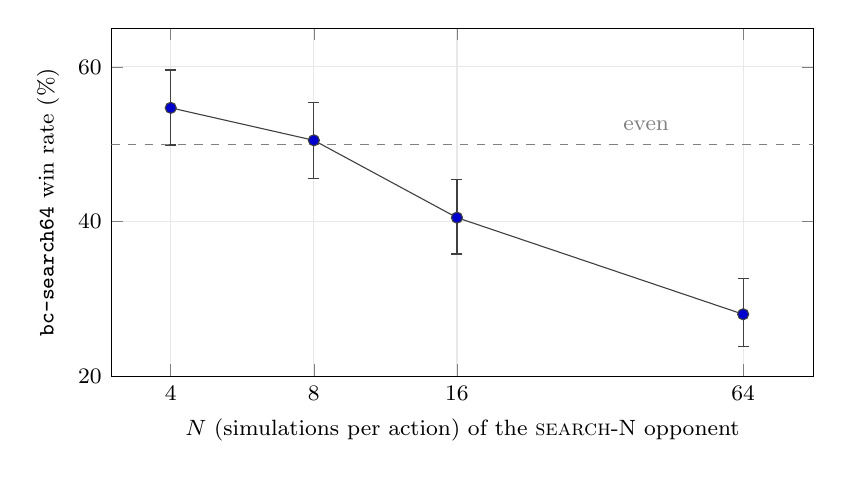
\begin{tikzpicture}
\begin{axis}[
  width=10.5cm, height=6cm,
  xlabel={$N$ (simulations per action) of the \searchn{N} opponent},
  ylabel={\texttt{bc-search64} win rate (\%)},
  xmode=log, log basis x=2, xmin=3, xmax=90,
  ymin=20, ymax=65, xtick={4,8,16,64},
  xticklabels={4,8,16,64},
  grid=major, grid style={gray!18},
  tick label style={font=\footnotesize}, label style={font=\footnotesize},
]
\addplot+[mark=*, mark size=2pt, color=black!75, error bars/.cd, y dir=both, y explicit]
table[x=n, y=w, y error minus=em, y error plus=ep, row sep=\\] {
n w em ep \\
4  54.7 4.8 4.9 \\
8  50.5 4.9 4.9 \\
16 40.5 4.7 4.9 \\
64 28.0 4.2 4.6 \\
};
\draw[dashed, gray] (axis cs:3,50) -- (axis cs:90,50);
\node[font=\footnotesize, gray] at (axis cs:40,52.4) {even};
\end{axis}
\end{tikzpicture}
\caption{How to read ladder strength. The distilled student crosses $50\%$ between $N=8$ and $N=16$, so its ladder strength is $\approx8$. Every PPO policy we trained lies left of $N=4$. An entrant's first milestone is to place a point to the right of $N=16$.}
\label{fig:ladder}
\end{figure}

\section{The Challenge Areas}
\label{sec:challenges}

These are the five problems we believe stand between the present state and an agent that plays \textit{Magic}. Each is stated with the current best result, an entry criterion precise enough to be aimed at, and our reason for thinking it is now tractable. They are ordered by how directly a newcomer can start.

\challenge{Beat the search ladder}{ch:ladder}

\textbf{Statement.} Produce a policy that, at inference time and without search, has ladder strength $N\ge16$.

\textbf{Current best.} \texttt{bc-search64}, at $N\approx8$, for \$0.66. Everything trained by RL from scratch: $N\lesssim1$.

\textbf{Entry criterion.} Beat \searchn{16} head-to-head over $\ge400$ seat-balanced games with a Wilson lower bound above $50\%$, at $<10$\,ms per decision and $<\$5$ of training. Report ladder strength, dollars, and milliseconds.

\textbf{Why it is tractable.} One round of the dumbest possible distillation --- argmax behavior cloning, no DAgger, no value head, no soft targets, one iteration --- already moved the trained frontier from $N\lesssim1$ to $N\approx8$. Expert iteration \citep{anthony2017exit,silver2018alphazero}, in which the student is fed back as the rollout policy, is the obvious next move and has not been run. We would be surprised if it did not clear $N=16$.

\challenge{Model the belief state}{ch:belief}

\textbf{Statement.} Replace uniform determinization with a learned posterior over the opponent's hidden state, and demonstrate that it improves play at a matched simulation budget.

\textbf{Current best.} None. \texttt{determinize()} draws uniformly from the opponent's unseen pool. This is an exactly correct posterior on turn one and a progressively worse one thereafter.

\textbf{Entry criterion.} A belief model $b(\text{hand} \mid \text{public history})$ that (i) beats the uniform prior in held-out log-likelihood of the true opponent hand, and (ii) when substituted into \texttt{determinize}, yields a searcher that beats an equal-simulation uniform searcher over $\ge400$ seat-balanced games.

\textbf{Why it is tractable, and why we think it is the best problem here.} In constructed \textit{Magic} both decklists are public. The hidden state is therefore a distribution over multisets drawn from a \emph{known, small} pool --- not the abstraction problem poker required. The training signal is free: self-play games reveal the true hand at showdown, so supervised learning applies directly. And the engine already isolates the intervention to a single function, so the experiment is a substitution, not a rewrite. The pathology this attacks --- strategy fusion \citep{frank1998bridge}, in which the searcher assumes it will know the opponent's hand at every future node and therefore cannot value information or represent \textit{Counterspell} as a \emph{threat} rather than a card --- is the reason our search plateaus. ReBeL \citep{brown2020rebel} and ISMCTS \citep{cowling2012ismcts} are the reference points.

\challenge{Long-horizon credit assignment without priors}{ch:credit}

\textbf{Statement.} Train an agent from terminal reward alone to ladder strength $N\ge16$.

\textbf{Current best.} Terminal-only PPO reaches $75.5\%$ against random (best of three seeds, \$0.14) but has never been placed on the ladder. We expect it is below $N=4$.

\textbf{Entry criterion.} As stated, with the \emph{terminal-only} reward. Shaped rewards are disqualifying, for the reason below.

\textbf{Why it is hard, and why the obvious escape is closed.} A game surfaces $117$--$194$ decisions; the GAE credit window is $\approx16.8$ steps. The natural response is dense shaping, and we spent the project's first year on exactly that. It was a mistake: per-event shaping is \emph{worse than no shaping at all} (\S\ref{sec:pitfalls}), because it is not a learning aid but a \emph{prior}, and it encoded the strategy of a creature deck into an agent playing a control deck. Potential-based shaping \citep{ng1999shaping} is policy-invariant and therefore, as theory predicts, does nothing: it ties terminal-only within noise. So the horizon must be closed architecturally --- by value functions that see further, by search-derived targets, by hierarchy --- and none of that has been tried here.

\challenge{Compositional generalization over an open card pool}{ch:pool}

\textbf{Statement.} Train an agent that plays competently with cards it has never seen.

\textbf{Current best.} None. Our observation encoder represents cards as hand-rolled feature vectors: six type flags, twelve keyword flags, power/toughness/mana value, three tribal tags. A card outside that vocabulary is unrepresentable.

\textbf{Entry criterion.} Hold out the ten-card modern slice (\texttt{cardsets/tla.rs}), train on the remaining pool, and evaluate zero-shot on decks containing the held-out cards. Beat a policy trained from scratch on the same held-out decks at equal cost.

\textbf{Why it is tractable now.} \textit{Magic} cards are natural-language rules text with a formal denotation. The architecture already scores actions by reference to the \emph{objects} they act on, so the card representation is a swappable leaf: replace the feature vector with a text encoder and the policy inherits compositional structure for free. This is the challenge on which the difference between ``a card game'' and ``\textit{Magic}'' entirely rests, and it is the one we consider most likely to be solved by someone outside game AI.

\challenge{Scale the rules substrate}{ch:rules}

\textbf{Statement.} Grow the engine from 35 cards toward a playable cube without losing throughput or correctness.

\textbf{Current best.} 35 cards, 106 rules-cited tests, $1.8\times10^{5}$ steps/s. Layers, replacement and prevention effects, mulligans, multi-block combat, and floating-mana choice are all absent.

\textbf{Entry criterion.} Implement a CR slice (layers being the hard one), keep the rules suite green, and hold $\ge10^{5}$ steps/s at 16 environments.

\textbf{Why it matters more than it looks.} This is the least glamorous challenge and the one that gates the other four. Our trigger substrate (\S\ref{sec:triggers}) is a bet that triggered abilities decompose into subjects, predicates, and composable effects; that bet is currently supported by 35 cards and no adversary. Layers --- \textit{Magic}'s continuous-effect resolution order --- is the standard place where naive engines die, and it is where we expect ours to. We would rather someone discover that on purpose.

\medskip
\noindent Two further problems we consider necessary but not yet challenge-shaped: \textbf{an opponent worth beating} (every number in this paper is anchored on a uniform random opponent or our own prior policies --- there is no self-play population, no Elo, no human evaluation), and \textbf{deck construction}, which is the real game and which we have not touched.

\section{Calibration Findings, or: What This Domain Will Do To You}
\label{sec:pitfalls}

Table~\ref{tab:refuted} lists eight claims this project acted on and the evidence that killed each. We publish it because six of the eight were used to justify a design decision, every one was originally established by a cheap unbalanced single-seed measurement, and every one survived for months because it was never the thing under test. An entrant who adopts the protocol in \S\ref{sec:protocol} will not rediscover them; an entrant who does not, will.

\begin{table}[H]
\centering\small
\begin{tabular}{p{6.2cm}p{2.1cm}p{5.4cm}}
\toprule
\textbf{Claim we acted on} & \textbf{Killed by} & \textbf{What was actually true} \\
\midrule
``The agent wins $82\%$ against random.'' & seat balance & It was on the play. Random wins $94\%$ on the play. \\
``Terminal reward fails; it causes pass-collapse.'' & replication & Does not replicate on either deck. Terminal-only is among our best recipes. \\
``Dense shaping is needed: the GAE horizon is $6\times$ too short.'' & \S\ref{sec:pitfalls} & Shaping is net harmful. It is a prior, not an aid. \\
``$\texttt{cast\_when\_able}\ge0.70$ marks a healthy policy.'' & \intdeck & Sign-flips once the deck has interaction. Good policies cast \emph{less}. \\
``Initialization variance is catastrophic ($13$--$89\%$).'' & seat balance & A seat$\times$init interaction. Balanced: $48.2$--$51.7\%$; all CIs cover $50\%$. \\
``Most decisions are trivial and auto-passed.'' & profiling & Only $12.4\%$ collapse. Combat is $58\%$ of real decisions. \\
``The environment is the bottleneck.'' & profiling & Inference costs $72\times$ the environment step. \\
``The interactive deck surfaces more decisions.'' & profiling & They fall to $0.60\times$. \\
\bottomrule
\end{tabular}
\caption{Eight claims, and their disposition. The fix in every case was a \$0 protocol change --- balance the seat, run 400 games, write the prediction down first --- not an algorithmic one.}
\label{tab:refuted}
\end{table}

Two of these deserve their own statement, because they are findings about the domain rather than about us.

\paragraph{Shaping is a prior, and it will be the wrong one.} Three reward regimes, three seeds each, 400 seat-balanced games:

\begin{center}\small
\begin{tabular}{lccc}
\toprule
Reward & Mean win \% & Range & \texttt{cast\_when\_able} \\
\midrule
Per-event shaping (our founding recipe) & $52.4$ & $43.2$--$58.3$ & $0.88$--$0.95$ \\
Potential-based $\Phi$ & $\mathbf{69.5}$ & $65.2$--$75.0$ & $0.35$--$0.38$ \\
Terminal-only & $66.7$ & $60.0$--$75.5$ & $0.15$--$0.29$ \\
\bottomrule
\end{tabular}\\[2pt]
{\footnotesize 400 seat-balanced games vs.\ uniform random, \intdeck. Potential-$\Phi$ and terminal-only are within noise of each other.}
\end{center}

Every potential-shaped seed beats every per-event seed, with non-overlapping intervals. Terminal-only ties potential-$\Phi$ --- exactly as \citet{ng1999shaping} predict, since $\gamma\Phi(s')-\Phi(s)$ is policy-invariant and therefore does no work. And the pass-collapse pathology that motivated dense shaping in the first place \emph{does not replicate}. The right amount of shaping in this domain is approximately zero.

\paragraph{The deck is the probe.} The most informative number above is the last column. The \emph{same} terminal-only reward yields $\texttt{cast\_when\_able}\approx0.99$ on \stddeck, where casting every creature on sight is correct, and $0.15$--$0.29$ on \intdeck, where holding instants is correct. The unshaped policy adapts to the deck; the shaped policy cannot. Any entrant claiming a learned policy should report this pair, because a single number cannot distinguish strategy from habit.

\section{Getting Started}

The repository contains the engine, the learner, the search player, the distillation harness, the evaluation protocol, and every experiment report backing the numbers in this paper.

\begin{itemize}\itemsep1pt
\item \texttt{managym/} --- the Rust engine and its 106 rules-cited tests. \texttt{cargo test}.
\item \texttt{manabot/} --- Gymnasium wrapper, PPO, \texttt{FlatMCPlayer}, distillation.
\item \texttt{manabot/verify/} --- the seat-balanced evaluation harness. Use this; do not write your own.
\item \texttt{reports/} --- one file per pre-registered cycle, with raw data in \texttt{reports/data/}.
\item \texttt{docs/rules\_coverage.yaml} --- machine-tracked scope. If your card needs a rule not listed here, it is Challenge \ref{ch:rules}.
\end{itemize}

The fastest path to a result: reproduce \searchn{16} against random (an afternoon, \$0), then place your own policy on the ladder. If it lands right of $N=16$, you have beaten this paper.

\section{Conclusion}

We set out to train an agent to play \textit{Magic: The Gathering}, and what we built instead was the apparatus for finding out whether anyone has. The engine is fast and correct within a stated subset; determinization is native, so imperfect-information search is one call; the protocol is calibrated, and calibrating it invalidated most of what we previously believed. The baselines are honest, and they say that a search costing nothing to train and seven milliseconds to run defeats every policy we produced, and that distilling that search is six times more cost-effective than reinforcement learning from scratch.

That last sentence is the state of the art, and it is an embarrassment to the learning literature rather than to search. The five challenges in \S\ref{sec:challenges} are the ways out of it, and the belief-modeling problem in particular strikes us as one of the cleanest open problems in imperfect-information games: a hidden state that is exactly enumerable, a free supervision signal, and a single function to replace. The instrument is built. The measurements are calibrated. Almost none of the science has been done.

\paragraph{Reproducibility.} All experiments are recorded under \texttt{reports/} with raw data in \texttt{reports/data/}. Provenance commits: \texttt{e38f20b} (cost basis), \texttt{b884038} (decision profile), \texttt{f019e7a} (seat-balanced baselines). Win-rate intervals are Wilson $95\%$.

\bibliographystyle{plainnat}
\bibliography{refs}

\end{document}
